%!TEX root = ../Thermodynamik II (LTNT).tex

\section{Erzwungene Konvektion an um\-ström\-ten Kör\-pern} % (fold)
	\subsection{Das Grenzschichtproblem an der ebenen Wand} % (fold)
		Randbedinungen:
		\begin{gather*}
			u(0) = 0\,,\quad v(0) = 0\,,\quad T(0) = T_W \\
			u(\infty) = u_\infty\,,\quad v(\infty) = 0\,,\quad T(\infty) = T_\infty\,,\quad p(\infty) = p_\infty
		\end{gather*}

		\subsubsection{Die Geschwindigkeitsgrenzschicht} % (fold)
			\emphequation{gather*}{
				\frac{\partial u}{\partial x} + \frac{\partial v}{\partial y} = 0 \tag{Kontinuität} \\
				u \cdot \frac{\partial u}{\partial x} + v \cdot \frac{\partial u}{\partial y} = \nu \frac{\partial^2 u}{\partial y^2} \tag{$x$-Impulsgleichung}
			}
			wobei $\nu = \mu / \rho$ und mit den Randbedingungen:
			\[
				u(0) = v(0) = 0\,,\quad u(y \to \infty) = U_\infty
			\]
		% subsubsection die_geschwindigkeitsgrenzschicht (end)

		\subsubsection{Die Temperaturgrenzschicht} % (fold)
			Es gilt $\delta_T \gg \delta_u$. Durch Vernachlässigung der Wärmeleitung in $x$-Richtung, folgt:

			\emphequation{equation}{\label{eq:konvektion}
				\begin{split}
					\frac{\partial u}{\partial x} + \frac{\partial v}{\partial y} &= 0 \\%tag{Kontinuität} \\
					u \cdot \frac{\partial u}{\partial x} + v \cdot \frac{\partial u}{\partial y} &= \nu \frac{\partial^2 u}{\partial y^2} \\%tag{$x$-Impulsgleichung} \\
					u \cdot \frac{\partial T}{\partial x} + v \cdot \frac{\partial T}{\partial y} &= a \frac{\partial^2 T}{\partial y^2} %\tag{Energie}
				\end{split}
			}
			mit den Randbedingungen:
			\begin{align*}
				y = 0\text{:} \quad & u(0) = v(0) = 0 \,,\quad T(0) = T_W \\
				y \to \infty\text{:} \quad & u(y \to \infty) = U_\infty \,,\quad T(y \to \infty) = T_\infty \\
				x = 0 \ (\forall y)\text{:} \quad & u = U_\infty \,,\quad T = T_\infty
			\end{align*}
		% subsubsection die_temperaturgrenzschicht (end)
	% subsection \textsc{das_grenzschichtproblem_an_der_ebenen_wand} (end)

	\subsection{Die Grössenordnungslösung} % (fold)
		Dimensionslose Zahlen:
		\begin{description}
			\item[Reynolds-Zahl:] $\mathrm{Re} = \frac{U_\infty \, L}{\nu} = \frac{\rho\, U_\infty \, L}{\mu} = \frac{\text{Massenträgheit}}{\text{Zähigkeit}}$
			\item[Prandtl-Zahl:] $\mathrm{Pr} = \frac{\nu}{a} = \frac{\mu c}{\lambda}
				= \frac{\text{Zähigkeit}}{\text{Wärmetransport}}$
			\item[Peclet-Zahl:] $\mathrm{Pe} = \mathrm{Re} \cdot \mathrm{Pr} = \frac{U_\infty \, L}{a} = \frac{\text{Massenträgheit}}{\text{Wärmetransport}}$
			\item[Nusselt-Zahl:] $\mathrm{Nu} = \frac{\overline\alpha \, L}{\lambda}$
		\end{description}
		wobei
		\begin{align*}
			\nu &= \frac{\mu}{\rho} \\
			a &= \frac{\lambda}{\rho c}
		\end{align*}

		\subsubsection{Strömungswiderstand} % (fold)
			Abschätzung der Dicke der Grenzschicht:
			\[
				\delta_u \approx \parens{
					\frac{\nu \cdot L}{U_\infty}
				}^{\nicehalf}
				\qquad \Rightarrow \qquad
				\frac {\delta_u} L \approx \mathrm{Re}_L^{-\nicehalf}
			\]

			Abschätzung der auftretenden Schubspannung:
			\[
				\tau_W \approx \rho \cdot U_\infty^2 \cdot \mathrm{Re}_L^{-\nicehalf} = c_f \cdot \frac \rho 2 \cdot U_\infty^2
			\]
			mit dem \textbf{Widerstandsbeiwert}
			$
				c_f = 2 \cdot \mathrm{Re}_L^{-\nicehalf}
			$

			Kraftwirkung:
			\[
				F \approx \rho \cdot U_\infty^2 \cdot W \cdot L \cdot \mathrm{Re}_L^{- \nicehalf}
			\]
		% subsubsection strömungswiderstand (end)

		\subsubsection{Wärmeübertragung} % (fold)
			\paragraph{Falls $\delta_u \ll \delta_T$} % (fold)
				\[
					\frac{\delta_T}{L} \approx \mathrm{Pe}^{- \nicehalf}
				\]
				Forderung: $\mathrm{Pr} \ll 1$

				Abschätzung des Wärmeübergangskoeffizienten:
				\[
					\overline\alpha \approx \frac{\lambda}{L} \cdot \mathrm{Pr}^{\nicehalf} \cdot \mathrm{Re}_L^{\nicehalf}
				\]
				Wärmestrom zwischen einer Wand der Breite $W$ und dem Fluid:
				\[
					\dot q = L \cdot W \cdot \overline\alpha \parens{T_W - T_\infty}
					\approx W \cdot \parens{T_W - T_\infty} \cdot \lambda \cdot \mathrm{Pr}^{\nicehalf} \cdot \mathrm{Re}^{\nicehalf}
				\]
			% paragraph fall_delta_u_ll_delta_t_ (end)

			\paragraph{Falls $\delta_u \gg \delta_T$} % (fold)
				\[
					\frac{\delta_T}{L} \approx \mathrm{Pr}^{- \nicefrac{1}{3}} \cdot \mathrm{Re}_L^{-\nicehalf}
				\]
				Forderung: $\mathrm{Pr} \gg 1$
				\begin{align*}
					\overline\alpha &\approx \frac \lambda L \cdot \mathrm{Pr}^{\nicefrac 1 3} \cdot \mathrm{Re}_L^{\nicehalf} \\
					\dot q &\approx W \cdot \parens{T_W - T_\infty} \cdot \lambda \cdot \mathrm{Pr}^{\nicefrac 1 3} \cdot \mathrm{Re}_L^{\nicehalf}
				\end{align*}
			% paragraph fall_delta_u_gg_delta_t_ (end)
		% subsubsection wärmeübertragung (end)
	% subsection die_grössenordnungslösung (end)

	\subsection{Die integrale Näherung} % (fold)
		\subsubsection{Integralgleichungen} % (fold)
			\begin{align*}
				\Diff{}{x} \int_0^{\delta_u} u \cdot \parens{ u - U_\infty } \diff y &= - \nu \cdot \parens{ \frac{\partial u}{\partial y} }_{y=0} \\
				\Diff{}{x} \int_0^{\delta_T} u \cdot \parens{ T - T_\infty } \diff y &= - a \cdot \parens{ \frac{\partial T}{\partial y} }_{y=0}
			\end{align*}
		% subsubsection integralgleichungen (end)

		\subsubsection{Lösung mit linearen Grenzschichtprofilen} % (fold)
			Voraussetzung: $\mathrm{Pr} > 1$, d.h.~$\delta_u > \delta_T$
			\begin{align*}
				\frac{u}{U_\infty} &= \frac{y}{\delta_u} \quad & y<\delta_u \\
				\frac{T-T_W}{T_\infty-T_W} &= \frac{y}{\delta_T} \quad & y<\delta_T
			\end{align*}

			Dicke der Grenzschicht, welche sich proportional zu $\sqrt x$ ausdehnt:
			\begin{align*}
				\delta_u &= \sqrt{\frac{12 \cdot \nu}{U_\infty} \cdot x} \qquad \text{mit} \quad \mathrm{Re}_x = \frac{x \cdot U_\infty}{\nu} \\
				\frac {\delta_u} x &= \sqrt{\frac{12}{\mathrm{Re}_x}} = 3.464 \cdot \mathrm{Re}_x^{-\nicehalf}
			\end{align*}

			Wandschubspannung bei bekannter Grenzschichtdicke:
			\[
				\tau_W = \mu \cdot \parens{\Diff u y}_{y=0} = \mu \cdot \frac{U_\infty}{\delta_u} = \frac{\rho \cdot U_\infty^2}{\sqrt{12 \cdot \mathrm{Re_x}}}
			\]

			Dimensionloser Widerstandsbeiwert:
			\[
				c_f = \frac{\tau_W}{\half \cdot \rho \cdot U_\infty^2} = 0.577 \cdot \mathrm{Re}_x^{-\nicehalf}
			\]

			Entwicklung der Temperaturgrenzschicht:
			\[
				\frac{\delta_T}{x} = \frac{\delta_u}{x} \cdot
					\mathrm{Pr}^{-\nicefrac 1 3} = 3.464 \cdot \mathrm{Re}_x^{-\nicehalf}
					\cdot \mathrm{Pr}^{-\nicefrac 1 3}
			\]

			Wärmeübergangskoeffizient:
			\begin{align*}
				\dot q_W'' &= -\lambda \cdot \left. \Diff T y \right|_{y=0} = - \lambda \cdot \frac{T_W - T_\infty}{\delta_T} \\
				&= \frac \lambda x \cdot 0.289 \cdot \mathrm{Re}_x^{\nicehalf} \cdot \mathrm{Pr}^{\nicefrac 1 3} \cdot \parens{T_W - T_\infty} \\
				\alpha &= \frac \lambda x \cdot 0.289 \cdot \mathrm{Re}_x^{\nicehalf} \cdot \mathrm{Pr}^{\nicefrac 1 3}
			\end{align*}
		% subsubsection lösung_mit_linearen_grenzschichtprofilen (end)
	% subsection die_integrale_näherung (end)

	\subsection{Exakte Lösung} % (fold)
		\paragraph{Die Geschwindigkeitsgrenzschicht} % (fold)
			\begin{align*}
				\delta_u &= 4.92 \cdot x \cdot \mathrm{Re}_x^{-\nicehalf} \\
				\frac{\delta_u}{\delta_T} &= \mathrm{Pr}^{\nicefrac 1 3} \\
				c_{fx} &= 0.664 \cdot \mathrm{Re}_x^{-\nicehalf} \\
				\overline c_{fx} &= 1.328 \cdot \mathrm{Re}_L^{-\nicehalf} \\
				F_W &= \overline\tau_L \cdot W \cdot L
			\end{align*}
		% paragraph die_geschwindigkeitsgrenzschicht (end)

		\paragraph{Die Temperaturgrenzschicht} % (fold)
			\begin{align*}
				\mathrm{Nu}_x &= \frac{\alpha \cdot x}{\lambda} = 0.332 \cdot \mathrm{Re}_x^{\nicehalf} \cdot \mathrm{Pr}^{\nicefrac 1 3} & \mathrm{Pr} > 0.6 \\
				\mathrm{Nu}_x &= \frac{\alpha \cdot x}{\lambda} = 0.565 \cdot (\mathrm{Re}_x\vphantom{1^2} \cdot \mathrm{Pr})^{\nicehalf} & \mathrm{Pr} < 0.6 \\
				\mathrm{Nu} &= \frac{0.3387 \cdot \mathrm{Re}_x^{\nicehalf} \cdot \mathrm{Pr}^{\nicefrac 1 3}}{\left[
					1 + \parens{
						0.0468 / \mathrm{Pr}
					}^{\nicefrac 2 3}
				\right]^{\nicefrac 1 4}} & \mathrm{Pe}_x = \mathrm{Re}_x \cdot \mathrm{Pr} > 100
			\end{align*}

			\emphequation{equation*}{
				\overline{\mathrm{Nu}} = 2 \cdot \mathrm{Nu}_L \quad \Rightarrow \quad
				\overline \alpha(L)
			}

		% paragraph die_temperaturgrenzschicht (end)
	% subsection exakte_lösung (end)

	\subsection{Turbulente Strömung} % (fold)
		Die in der Zeit sich ändernden Variablen werden durch einen Mittelwert und einen fluktuirenden Anteil dargestellt:
		\[
			u = \overline u + u'\,,\ v = \overline v + v'\,,\ w = \overline w + w'\,,\ P = \overline P + P'\,,\ T = \overline T + T'
		\]

		Gesetze:
		\begin{align*}
			c_{fx} &= 0.0592 \cdot \mathrm{Re}_x^{-\nicefrac 1 5} & \mathrm{Re}_x \le 10^7 \\
			\mathrm{Nu}_x &= 0.0296 \cdot \mathrm{Re}_x^{\nicefrac 4 5} \cdot \mathrm{Pr}^{\nicefrac 1 3} \\
			\mathrm{Re}_x &= \frac{U_\infty \cdot x}{\nu} \\
			\mathrm{Nu} &= \frac{\alpha \cdot x}{\lambda}
		\end{align*}

		Die kritische Reynolds-Zahl für Strömungen über eben Flächen, wo der Umschlag zur turbulenten Strömung erfolgt, liegt im Bereich $(1\text-2)\cdot 10^5$.

		Die Reynolds-Zahl wächst mit zunehmendem Abstand zur Anströmkante, so dass ab einem gewissen $x_\text{krit}$ sich die turbulente Strömung ausgebildet hat:
		\[
			\mathrm{Re}_{x\text{,krit}} = \frac{x_\text{krit} \cdot U_\infty}{\nu}
		\]
	% subsection turbulente_strömung (end)

	\subsection{Wärmeübergang an umströmten Körpern} % (fold)
		\subsubsection{Quer angeströmte zylindrische Körper} % (fold)
			\[
				\overline{\mathrm{Nu}}_D = \frac{\overline\alpha \cdot D}{\lambda} = C \cdot \mathrm{Re}_D^m \cdot \mathrm{Pr}^{\nicefrac 1 3}
			\]
			$\rho$, $\mu$ (resp.~$\nu$) und $\lambda$ sind temperaturabhängig. Für die Temperatur wird die Filmtemperatur (Mittelwert über die Grenzschicht) eingesetzt:
			\[
				T_\text{Film} = \half (T_W + T_\infty)\,,\quad \mathrm{Re}_D = \frac{U_\infty \cdot D}{\nu(T_F)}\,,\quad \mathrm{Pr} = \frac{\nu(T_F)}{a(T_F)}
			\]

			Zahlenwerte für einen Zylinder mit \emph{Durchmesser} $D$:
			\begin{center}
				\begin{tabular}{r@{}l@{$\:-\:$}rcr@{.}lcr@{.}l}
					\toprule
					\multicolumn{3}{c}{$\boldsymbol{\mathrm{Re}_D}$} && \multicolumn{2}{c}{$\boldsymbol C$} && \multicolumn{2}{c}{$\boldsymbol m$} \\
					\midrule
					     0 & .4 & 4       && 0 & 989 && 0 & 330 \\
					     4 &    & 40      && 0 & 911 && 0 & 385 \\
					    40 &    & 4'000   && 0 & 683 && 0 & 466 \\
					 4'000 &    & 40'000  && 0 & 193 && 0 & 618 \\
					40'000 &    & 400'000 && 0 & 027 && 0 & 805 \\
					\bottomrule
				\end{tabular}
			\end{center}

			Selbe Analogie für Stäbe mit nicht kreisförmigen Querschnitten:
			\begin{center}
				\begin{tabular}{@{}p{.6cm}@{}m{.9cm}@{}m{.15cm}cr@{$\:-\:$}lcr@{.}lcr@{.}l@{}}
					\toprule
					\multicolumn{3}{c}{\textbf{Geometrie}} && \multicolumn{2}{c}{$\boldsymbol{\mathrm{Re}_D}$} && \multicolumn{2}{c}{$\boldsymbol C$} && \multicolumn{2}{c}{$\boldsymbol m$} \\
					\midrule
					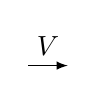
\begin{tikzpicture}[>=latex,scale=.5]
	\draw[->] (0,0) -- (1,0) node[pos=.5,above]{$V$};
\end{tikzpicture}&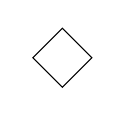
\begin{tikzpicture}[>=latex,scale=.75]
	\begin{scope}[rotate=45,scale=0.707107,xshift=-.5cm,yshift=-.5cm]
		\draw (0,0) -- (1,0) -- (1,1) -- (0,1) -- cycle;
	\end{scope}
	% center
	\begin{scope}[scale=0.57735,xshift=-.5cm,yshift=-.866cm,opacity=0]
		\draw (0,0) -- (1,0) -- ++(60:1) -- ++(120:1) -- ++(180:1) -- ++(240:1) -- ++(300:1) -- cycle;
	\end{scope}
\end{tikzpicture}& \begin{tikzpicture}[>=latex,scale=.75]
	\draw (0,0) -- (0,1) node[pos=.5,right]{$D$};
	\draw (-.075,0) -- (.075,0);
	\draw (-.075,1) -- (.075,1);
\end{tikzpicture} && $5 \cdot 10^3$ & $10^5$ && 0&246 && 0&588 \\
					\midrule
					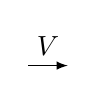
\begin{tikzpicture}[>=latex,scale=.5]
	\draw[->] (0,0) -- (1,0) node[pos=.5,above]{$V$};
\end{tikzpicture}&\begin{tikzpicture}[>=latex,scale=.75]
	\begin{scope}[xshift=-.5cm,yshift=-.5cm]
		\draw (0,0) -- (1,0) -- (1,1) -- (0,1) -- cycle;
	\end{scope}
	% center
	\begin{scope}[scale=0.57735,xshift=-.5cm,yshift=-.866cm,opacity=0]
		\draw (0,0) -- (1,0) -- ++(60:1) -- ++(120:1) -- ++(180:1) -- ++(240:1) -- ++(300:1) -- cycle;
	\end{scope}
\end{tikzpicture} & \begin{tikzpicture}[>=latex,scale=.75]
	\draw (0,0) -- (0,1) node[pos=.5,right]{$D$};
	\draw (-.075,0) -- (.075,0);
	\draw (-.075,1) -- (.075,1);
\end{tikzpicture} && $5 \cdot 10^3$ & $10^5$ && 0&102 && 0&675 \\
					\midrule
					\multirow{2}{*}{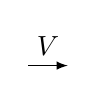
\begin{tikzpicture}[>=latex,scale=.5]
	\draw[->] (0,0) -- (1,0) node[pos=.5,above]{$V$};
\end{tikzpicture}}&\multirow{2}{*}{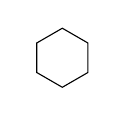
\begin{tikzpicture}[>=latex,scale=.75]
	\begin{scope}[rotate=30,scale=0.5]
		\draw (0,0) -- (1,0) -- ++(60:1) -- ++(120:1) -- ++(180:1) -- ++(240:1) -- ++(300:1) -- cycle;
	\end{scope}
	% center
	\begin{scope}[scale=0.57735,xshift=-.5cm,opacity=0]
		\draw (0,0) -- (1,0) -- ++(60:1) -- ++(120:1) -- ++(180:1) -- ++(240:1) -- ++(300:1) -- cycle;
	\end{scope}
\end{tikzpicture}} &\multirow{2}{*}{\begin{tikzpicture}[>=latex,scale=.75]
	\draw (0,0) -- (0,1) node[pos=.5,right]{$D$};
	\draw (-.075,0) -- (.075,0);
	\draw (-.075,1) -- (.075,1);
\end{tikzpicture}} && $5 \cdot 10^3$ & $1.95 \cdot 10^4$ && 0&160 && 0&638 \\
					& & && $1.95 \cdot 10^4$ & $10^5$ && 0&0385 && 0&782 \\
					\midrule
					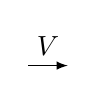
\begin{tikzpicture}[>=latex,scale=.5]
	\draw[->] (0,0) -- (1,0) node[pos=.5,above]{$V$};
\end{tikzpicture}&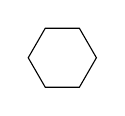
\begin{tikzpicture}[>=latex,scale=.75]
	\begin{scope}[scale=0.57735]
		\draw (0,0) -- (1,0) -- ++(60:1) -- ++(120:1) -- ++(180:1) -- ++(240:1) -- ++(300:1) -- cycle;
	\end{scope}
\end{tikzpicture} &\begin{tikzpicture}[>=latex,scale=.75]
	\draw (0,0) -- (0,1) node[pos=.5,right]{$D$};
	\draw (-.075,0) -- (.075,0);
	\draw (-.075,1) -- (.075,1);
\end{tikzpicture} && $5 \cdot 10^3$ & $10^5$ && 0&153 && 0&638 \\
					\midrule
					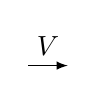
\begin{tikzpicture}[>=latex,scale=.5]
	\draw[->] (0,0) -- (1,0) node[pos=.5,above]{$V$};
\end{tikzpicture}&\begin{tikzpicture}[>=latex,scale=.75]
	\begin{scope}[xscale=.2]
		\begin{scope}[xshift=-.5cm,yshift=-.5cm]
			\draw (0,0) -- (1,0) -- (1,1) -- (0,1) -- cycle;
		\end{scope}
	\end{scope}
	% center
	\begin{scope}[scale=0.57735,xshift=-.5cm,yshift=-.866cm,opacity=0]
		\draw (0,0) -- (1,0) -- ++(60:1) -- ++(120:1) -- ++(180:1) -- ++(240:1) -- ++(300:1) -- cycle;
	\end{scope}
\end{tikzpicture} &\begin{tikzpicture}[>=latex,scale=.75]
	\draw (0,0) -- (0,1) node[pos=.5,right]{$D$};
	\draw (-.075,0) -- (.075,0);
	\draw (-.075,1) -- (.075,1);
\end{tikzpicture} && $4 \cdot 10^3$ & $1.5 \cdot 10^4$ && 0&228 && 0&731 \\
					\bottomrule
				\end{tabular}
			\end{center}

		% subsubsection quer_angeströmte_zylindrische_körper (end)

		\subsubsection{Die umströmte Kugel} % (fold)
			\[
				\overline{\mathrm{Nu}}_D = 2+(0.4 \cdot \mathrm{Re}_D^{\nicehalf} + 0.06 \cdot \mathrm{Re}_D^{\nicefrac 2 3}) \cdot \mathrm{Pr}^{0.4} \cdot \parens{\frac{\mu}{\mu_W}}^{\nicefrac 1 4}
			\]
			Gültigkeitsbereich:
			\[
				\begin{array}{r@{.}l@{\quad<\quad}c@{\quad<\quad}r@{}l}
					0&71 & \mathrm{Pr} & 380 & \\
					3&5 & \mathrm{Re}_D & 7&.6\cdot 10^4 \\
					1&0 & \frac{\mu}{\mu_W} & 3&.2
				\end{array}
			\]
			Der Bereich kleiner Reynolds-Zahlen ist von Bedeutung, da dieses Gesetz typischerweise auf Tropfen mit Durchmessern $< 100\si{\micro\metre}$ angewendet wird.
		% subsubsection die_umströmte_kugel (end)
	% subsection wärmeübergang_an_umströmten_körpern (end)
% section erzwungene_konvektion_an_umströmten_körpern (end)
